%
% File XCS224U_final_paper.tex
%

\documentclass[11pt,a4paper]{article}
\usepackage[hyperref]{acl2020}
\usepackage{times}
\usepackage{latexsym}
\usepackage{graphicx}
\renewcommand{\UrlFont}{\ttfamily\small}

% This is not strictly necessary, and may be commented out,
% but it will improve the layout of the manuscript,
% and will typically save some space.
\usepackage{microtype}

\aclfinalcopy % Uncomment this line for the final submission
%\def\aclpaperid{***} %  Enter the acl Paper ID here

%\setlength\titlebox{5cm}
% You can expand the titlebox if you need extra space
% to show all the authors. Please do not make the titlebox
% smaller than 5cm (the original size); we will check this
% in the camera-ready version and ask you to change it back.

\newcommand\BibTeX{B\textsc{ib}\TeX}

\title{Colors in Context: Grounded Language Understanding using Convolutional and Transformer Embeddings}

\author{
  Anton Gochev \\
  \texttt{gochev.anton@gmail.com} \\
  \And
  Jaro Habr \\
  \texttt{jaro.habr@gmail.com} \\
  \AND
  Yan Jiang \\
  \texttt{enaj1125@gmail.com} \\
  \And
  Samuel Kahn \\
  \texttt{samuelkahn@berkeley.edu} \\
}

\date{}

\begin{document}
\maketitle

\begin{abstract}

  In this work we present a new model for a grounded communication task; identifying colors  generated from descriptions. This task uses two recurrent neural network cells which act as the speaker generating utterances. We build on previous work and introduce two novel methods for embedding our recurrent neural network inputs; a convolutional encoder for colors and a transformer network for encoding utterances. We show that coupling these two encoders with a recurrent sequence-to-sequence architectures can sometimes achieve state-of-the-art results in both listener accuracy and BLEU score, but the gains are often minimal with a much great computational cost and highly prone to overfitting. In addition, our paper demonstrates that using complex encoders such as transformers or convolutional neural networks on small high dimensional datasets don't clearly outperform simpler models such as a Fourier Transform or GLoVe.


% \begin{itemize}
%   \item define current proposal, situate in context
%   \item summarize core findings
%   \item identify significance of work
% \end{itemize}

\end{abstract}
\section{Introduction}

In recent years, attention-based models and especially transformers have proven to be the best performing approaches in the area of natural language processing (NLP).

\par
In this paper, our core hypothesis is that transformers’ pretrained and contextual embeddings will enhance the word representations, therefore enhancing the performance of task of color description. We also hypothesise that using a convolutional neural network (CNN) to generate color embeddings will have a positive effect on the performance.  To test the hypothesis,  we applied pretrained and contextual word embeddings from BERT, RoBERTa, ELECTRA and XLNet models to the task, combined with a color representation produced by ResNet , and compare them to the baseline system developed in assignment 4 of the XCS224u course. We further define our core hypotheses into three parts and tested them in this work.

\par
The first hypothesis is pretrained and contextual embeddings will perform better than pretrained word representations like GloVe on the task.

\par
The second hypothesis is that the models in the first hypothesis can be further enhanced by replacing the original color representation with rich color representations produced by ResNet. Additionally, hyperparameters tuning could further  boost the model performance.

\par
The third hypothesis is that different combinations (addition, mean, etc.) of the transformer’s hidden layers will improve the performance of the whole system.

\par
We found that: 1) Complex color and text representations don’t necessarily perform better than the baseline model on the given task, 2) LSTM generally showed better performance than GRU as the sequence-to-sequence architecture, which is likely due to capturing the long-term dependencies of the utterances, 3) Hyperparameters (e.g, hidden dimensions) tuning also significantly enhanced model accuracy and Bleu score.

% \begin{itemize}
%   \item area of field of work
%   \item "The central hypothesis of this paper is..."
%   \item concepts, building blocks of the hypothesis
%   \item why \emph{this} hypothesis?
%   \item steps to address hypothesis
%   \item central findings of paper
% \end{itemize}
\section{Related Work}

\citep{monroe-2016-compositional} build a model that is capable of producing novel color descriptions (“greenish”, “bright”, "faded teal") not seen during training. This is a challenging task as color descriptions can be vague, compositionally complex and denotationally rich. They consider color generation as a grounded language modelling problem and present an effective approach to perform this task using LSTM RNN and color representations transformed with Fourier transformation used in computer vision for feature representations. The study of \citep{monroe-2017-colors} is continuation of the work of \citep{monroe-2016-compositional}. The autors create a much larger task-oriented dialog corpus \citep{moroe-2017-colors-reference-dataset} where a listener has identified a color based on short descriptions from a speaker. This dataset contains color descriptions using a variety of language use such as negations, comparatives, superlatives, metaphors, and shared associations. The authors show that a model, a combination of a listener RNN and a speaker RNN, performs better although both perform purely alone. They also observe significant improvement of the listener RNN with pragmatic reasoning and especially in the hardest cases: 1) contexts with very similar colors; 2) target colors that the referring expressions fail to identify.

\par
Another challening machine learning task that requires contextual grounding and complex language is the task of describing images. \citep{andreas-2016-reasoning} present a model with a feature-driven architecture using a simple NN listener and speaker. The model is capable of actively reasoning about the listener’s behaviour when selecting utterances describing images. It has to produce a pragmatic description of an image caption that is informative, fluent, concise and understanding the listeners’ behaviour. The model is able to outperform the baseline system by generating image descriptions that are correctly interpreted 17\% more often.

\par
Four different transformers that make use of attention which improve on different inefficiencies of BERT. To solve the data corruption and discrepancy problems of the BERT-based transformers caused by [MASK] token, XLNet uses an autoregressive language model, and ELECTRA uses a novel training scheme reminiscent of a Generative Adversarial Network (GAN). RoBERTa implements a new dynamic masking strategy to be able to pretrain on more data.

\par
The ability of humans to describe images with natural language and hence connect those two dimensions in a fluent way is the guiding motivation for the exploration of the multimodal space. The work by \citep{karpathy-2014-image_descriptions} focuses on generating concise descriptions from images by using deep neural networks. To create dense descriptions of visual data, the authors present a new multimodal recurrent neural network generative model which uses a region convolutional neural network (RCNN) pre-trained on ImageNet \citep{deng-2009-imagenet} to detect objects in every image. The generative model was trained to predict the next word given the previous context word and the probability distribution of the words in the vocabulary, denoting the start and end of the sequence with a special START and END token. In this context, the work of \citep{monroe-2017-colors} can be seen as a special case of image captioning, with the encoder part enriched with Fourier transformed color representation. Lastly, a more recent work published by \citep{openai-2020-dalle} presents a generative multimodal model called DALL·E, capable of generating or completing images from text. It uses a trained transformer to autoregressively model the text and image tokens as a single stream of data.

\par
In our work, we enhanced the color representation of the original model by \citep{monroe-2017-colors} with an encoder based on convolutional neural networks like ResNet-18 and encoded the word representations as pre-trained and contextual word embeddings based on transformer models like BERT, ELECTRA, RoBERTa or XLNet. Since ResNet-18 and ResNet-50 have been pre-trained on the ImageNet \citep{imagenet-2019-dataset}, we evaluate their embedded richer grounding color information compared to pure Fourier transformed color representations.

\section{Data}

We evaluate our models on the color dataset used in \citep{monroe-2017-colors}. This dataset was generated by playing reference games where the color descriptions were produced by human participants in the speaker role. On each round of the game, the speakers were presented with three color patches, one of which was selected to be the target color. The speakers were instructed to communicate this information to the listeners who were asked to click on one of the colors to complete the task \citep{monroe-2017-colors}.

\par
The dataset contains 49,025 examples in total and was split to train and test set with 46,994 and 2,031 examples respectively. Every dataset comprises examples containing three colors, one of them being the target color to be described and the other two being distractor colors. Every example belongs to one of three conditions: 1) \emph{close}, where all three colors are similar, 2) \emph{split}, where one of the colors is close to the target colors and 3) \emph{far}, where all three colors are far apart in the color space \citep{monroe-2017-colors}. Table \ref{table:colors} shows one example of each condition.

\begin{table}[ht]
\centering
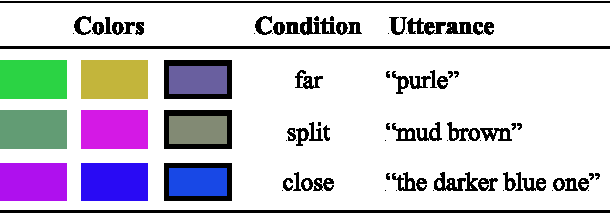
\includegraphics[width=\columnwidth]{assets/colors.pdf}
\caption[Colors]{Three color patches, represented using HLS values, are presented to the speaker. Each color patch set belongs to one of three conditions - far, split, close. The speakers describe the target color (marked with frame) to the listener (utterance).}
\label{table:colors}
\end{table}

\par
40.8\% of the \emph{train} dataset color descriptions use one word, 59.2\% use two or more with the majority being shorter than 14 words. All conditions are represented equally with 15,519 examples for the \emph{close}, 15,693 examples for the \emph{split} and 15,782 examples for the \emph{far} condition. The train dataset is further divided using 90/10 split while training.

\par
The \emph{test} dataset has a slightly different composition. 40.2\% of the color descriptions use one word, 54.6\% use two words and only 5.2\% use three or more words. The conditions are represented with 633 examples for the \emph{close}, 652 for the \emph{split} condition and 746 for the \emph{far} condition.
\section{Models}

This section describes the models in more detail.

\subsection{Target Architecture}
The following image depicts our target architecture developed for our experiments.

\begin{figure}[ht]
\centering
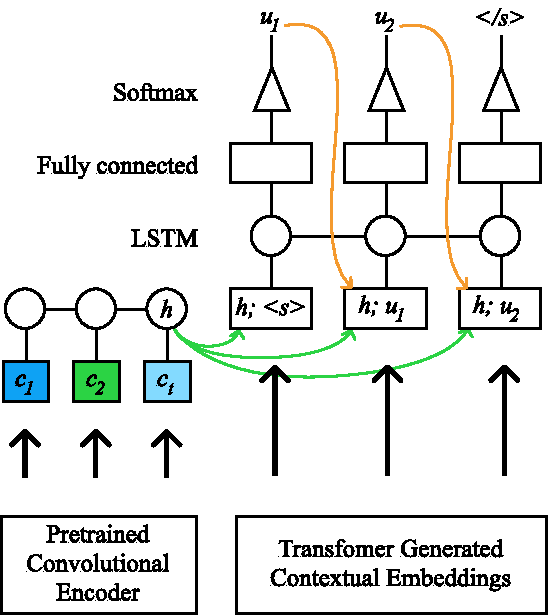
\includegraphics[width=\columnwidth]{assets/target_architecture.pdf}
\caption[Target Architecture]
{Target architecture with pre-trained convolutional encoder and transformer generated contextual word embeddings.}
\label{overview}
\end{figure}

\par
The above architecture consists of three core components. The pre-trained convolutional encoder is our method for extracting rich color embeddings. This could be any pre-trained convolutional model such as \texttt{VGG19} or \texttt{Resnet152}, it just requires that we use one of the last hidden layers before the softmax projection as our encode color embeddings. We use the last layer of \texttt{ResNet18} in our experiments.

\par
The transformer generated contextual embeddings are any word embeddings generated by a transformer. This could be embeddings generated by \texttt{ELECTRA}, \texttt{XLNet}, \texttt{BERT} or any other transformer variants. These are used to encode the words into a semantic vector space where their project will be dependent on their context. Some descriptions are single words, thus contextual information will not be encoded.

\par
The generated color and contextual word embeddings are then brought together using a standard sequence-to-sequence architecture. The color embeddings are sent through an RNN unit such as a Gated Recurrent Unit or Long Short Term Memory Unit. The target color is sent through the RNN layer last so that it’s information encoded in the hidden state is \emph{closest} to the decoder. The decoder, another RNN unit,  then takes the hidden encoder's last hidden layer input and starts to decode the input utterance. For each timestep of the decoder we concatenate the target colors embedding, generated by the \texttt{ResNet18}, with the input word. Once the output RNN reaches its specified stop token we stop generating text.

\subsection{Experiment Setup}
To address our hypotheses we use different model compositions which are based on our target architecture.

\textbf{Baseline}:
As a baseline model, we use our implementation of the encoder-decoder architecture model based on a single layer of GRU for both the encoder and decoder. The colors are encoded using Fourier transformation.

\textbf{Part one}:
We use Fourier encoded context colors with pre-trained and contextual embeddings from the following transformer models: \texttt{BERT}, \texttt{XLNet}, \texttt{ELECTRA}, \texttt{RoBERTa}.

\textbf{Part two}:
We use \texttt{ResNet} for contextual color representation while keeping the same model embeddings.

\textbf{Part three}:
We build on part two and combine different hidden layers of the transformer models. Namely, we concatenate the last four hidden layers, sum the last four hidden layers and extract the last and second-to-last hidden layer.
\section{Experiment}

Table INSERT TABLE NUMBER summarizes our results. We list our results in order of number of parameters in the model. This is a combination of trainable and untrainable parameters, as the core architecture of our models is generally a flavor of a recurrent neural network sequence-to-sequence model. The core architectural differences are captured by the method we use for embedding words and colors, while our encoder-decoder architecture generally stays the same. We use GRU as a default cell for all experiments. We also used an LSTM cell for the experiments that have shown best model performance to evaluate how a LSTM affects the performance of the models in comparison with GRU.

\par
We experimented with four different hidden dimensions (hidden\_size) for the RNN cells. We used 50 (default for all experiments) , 100, 150, 250 to determine what hidden dimensions will have the most positive effect on the model performance. Those experiments were conducted on models with RoBERTa, BERT, XLNet or ELECTRA pre-trained word embeddings and Fourier transformed or ResNet concatenated with Fourier transformed colour embeddings. A subset of the train dataset (8,000 records) was used for those experiments. We limited the number of experiments due to time and budget limitations. Finally, we trained and tested the best performing models with a hidden dimension of 250 as our experiments showed that a higher dimension has a positive effect on the model output.

\par
For example, for our simplest model (ID \#1) we use a fourier transform to project the colors from a 3-dimensional vector to a 54-dimensional vector. We use 50-dimensional pre-trained GLoVe embeddings to embed each word in the corpus as a distributed representation. We use a sequence-to-sequence model with a GRU cell acting as a color encoder and text decoder.  For this baseline model (and all models) we set the hidden dimension of the GRU to 50. From \citep{dey-2017-gru} there are a total of \[3*(n^2 + n*m +n)\] where n is the hidden dimension of the GRU and m is the input dimension to the cell. So for our encoder our number of trainable weights becomes:

\[3*(50^2 + 50*54 +50) = 15,150\]

\par
and for the decoder our number of weights becomes:

\[3*(50^2 + 50*50 +50) = 15,750\]

\par
For the entire architecture this totals to 30,900 trainable parameters. We note that we freeze the word embeddings and color embeddings in all models.

\par
Now for a more complex model that incorporates both transformer pre-trained or contextual word embeddings and color embeddings generated by a convolutional encoder, our number of trainable parameters increases. For a model that uses 768-dimensional BERT embeddings and 512-dimensional ResNet encoded color embeddings our trainable parameters for the encoder becomes:

\[3*(50^2 + 50*512 +50) = 84,450\]

\par
and for the decoder our number of weights becomes:

\[3*(50^2 + 50*768 +50) = 122,850\]

\par
This results in a total of 207,300 trainable parameters. The number of trainable parameters significantly increases for the experiments that we used hidden dimension of 250. For the aforementioned example the number of trainable parameters used in the encoder becomes:

\[3*(250^2 + 250*512 +50) = 571,650\]

\par
And for the decoder the number of weights becomes:

\[3*(250^2 + 250*768 +50) = 763,650\]

\par
We note that while the more complex models have more power to capture complex interactions, the large models have nearly seven times the number of trainable parameters leading to concerns of building models with high variance. We will discuss the effects of model size and overfitting further in our Analysis section.

\par
For all models we stop training after the validation performance has increased for 10 iterations in a row at a tolerance of \(10^-5\). We use the listener accuracy and the BLEU score to evaluate model performance.

\par
Listener accuracy and BLEU score are used for evaluating the performance of the models. The former allows us to evaluate the ability of the trained model to construct accurate colour description utterances based on the colours input.

\[c^{*} = argmax_{c \in C} P_{s} (utterance | c)\]

\par
where \(P_{s}\) is the describer model and \(C\) is the set of all permutations of all three colors in the color context. We take \(c^{*}\) to be a correct prediction if it is one where the target is in the privileged final position \citep{potts-2020-colors}.

\par
The listener's accuracy assesses the ability of the model to communicate with itself and this can lead to generating utterances that are far from proper English. BLEU score is used to ensure that this situation doesn’t happen.

\par
We consider both listener accuracy and BLEU score, with equal performance when evaluating the models and therefore, a model is consider better performing if both scores are higher.

\bigbreak
[table goes here]



% \bigbreak
% what to write:
% \begin{itemize}
%   \item explain how data and models work together for my experiments
%   \item show which models were eveluated
%   \item how models were trained
%   \item data pre-processing
%   \item which metrics were used
%   \item what are experimental outcomes
% \end{itemize}
\section{Analysis}

\subsection{Color Embeddings}

Intuitively we would think that making our architecture more complex and adding richer  embeddings would capture the nuances of generating utterances from color embeddings. We do demonstrate this is the case in certain architectures, but adding more complexity does not necessarily lead to better performance.

\par
We find that mapping our 3-dimensional color embeddings to 54 dimensions using a fourier transformation consistently performs the best. This is a surprising result as embedding our colors using a convolutional neural network, such as a residual network, embeds much richer semantic information. There are a few explanations for why this might be.

\par
The first explanation is that while residual networks can capture rich semantic information as we encode a color with it, it is not appropriate for embedding something as simple as a color. Each layer of convolutional neural networks are supposed to find lower level features in an input image, but with a solid color there are effectively no low level features to find. So it’s likely that using the residual network as a feature extractor is actually embedding unnecessary noise into each color. We should also note that the residual networks we use in our experiments were trained on the ImageNet dataset, which requires the network to model much more complicated visual semantics than classifying a single color would.

\par
Another explanation why embedding our colors using a residual network leads to worse performance is the increase in size of our input embeddings. Our color embedding sizes go from 54-dimensional to 512-dimensional which is a more the 9x increase in dimension. This could be too large a vector for our architectures to model without fitting to noise. Putting it  another way, we could be overfitting which is leading to very poor generalization. This is not out of the question as our models already have several thousand learnable parameters and adding more seems to consistently make our models perform worse.

\par
A third explanation as to why our convolutional color encoder did not perform well is that we must capture more than the last layer as the color embedding. Possible options would be the element-wise sum, max, or average of the last N layers as a feature extractor. Another possibility would be to concatenate the vectors to create an N*512 dimensional embedding, where N is the number of layers used in the feature extraction. This is a similar technique we use in our word embeddings, which we discuss in the following section.

\subsection{Pretrained and Contextual Embeddings}

Our use of pretrained and contextual embeddings, such as BERT, XLNet, RoBERTa and ELECTRA was motivated by a similar thought process as our color embeddings. We believed that using more powerful models that capture linguistic \& semantic information would lead to better performance. Our best performing models (ELECTRA and XLNet) using pretrained word embeddings, did not perform much better than using GloVe embeddings. AllMost contextual word embedding models performed worse than GloVe vectors. We used , especially when we actually use the contextual word embeddings output from the last layer, (or a combination of the last N layers, [CLS] sentence embedding, and concatenating the last layer or [CLS] and pretrained embeddings). In all cases we observed the latter leads to improving the performance of the model.

\par
We believe the explanation for this mostly lies in our dataset used for training. The 40.8\% of our examples only contain a single  word,, so using contextual word embeddings would not add as much value as if the dataset would have consisted of more complex color descriptions. Using contextual embeddings requires our downstream  model to be able to effectively learn the meaning of a word embedding given its context. But given our small dataset this is likely not a feasible task leading to overfitting or simply not enough complex data to capture the intricacies.

\par
Another possible explanation is that we are not producing the contextual embeddings in a way that properly captures the semantic information our model needs. Similar to the potential changes we could make to the color embedding, we could employ different methods of combining hidden layers embeddings for both the contextual word embeddings and the [CLS] sentence embedding. There are several methods we could use including the element-wise sum, max, or average of the last N layers as a feature extractor. This could include both the contextual word embeddings and the [CLS] sentence embeddings. We could even include the pretrainedstatic word embeddingswordtoken embeddings, but should note this would add a great deal of dimensionality to our models. This would increase the likelihood of building models with high variance.  We did explore this a bit with experiments resulting in poor performance, but we did not enumerate and experiment all the possible vectors and layer combinations that could potentially yield good performance.


\subsection{Sequence-to-Sequence Architecture}

We explored using two different types of RNN cells; a GRU and LSTM cell.  We found the LSTM to generally perform better than the GRU cell. The accuracy of the model using residual network color embeddings and pretrained token embeddings improved with over 0.40 and BLEU score improved with 0.1-0.33. The accuracy of the model using Fourier color embeddings and pretrained token embeddings improved slightly with a maximum of 0.03 but the BLEU score improved significantly with a maximum of 0.14. This is somewhat surprising as adding complexity to the other aspects of our models, such as the color embeddings and word embeddings, generally lead to worse performance.

\par
A possible explanation to this observation could be that the LSTM is inherently better at capturing long-term dependencies. This leads it to doing a better job in encoding the color representation in the last hidden state of the encoder. There are only three colors we must encode so it’s unlikely that we would get that much gain from an LSTM in the encoder. It is more likely that it is better capturing the long term dependencies of the utterances and producing utterances that are more coherent. This is reflected in the BLEU scores produced by architectures that include an LSTM cell.

\subsection{Hyperparameters Tuning}
We experimented mainly with setting different hidden dimensions for the RNN cells. Nearly in all experiments with the increase of the hidden dimension we observed an improvement of the accuracy and significant improvement of the BLEU score with hidden dimension set to 250 performing the best. As we limited our experiments to only four dimensions settings (50, 100, 150, 250) tested with a subset of the train data (8 000 records) and the best performing models it might be that a different hidden dimension size might lead to even better performance.

\par
It is possible that with the increase of the hidden dimension size the models are able to capture additional information via the significantly increased number of trained parameters. This could potentially lead to overfitting or a better performance of the model. Our data shows that the model had a slightly better performance with the dev dataset and significantly better performance with the test dataset. Consequently, we believe that the model is not overfitted but rather has captured additional information allowing it to perform better and produce significantly better English.

\subsection{Best Models Learning Efficiency}
We trained and evaluated the performance of our baseline model with GloVe, with ELECTRA and XLNet pretrained embeddings with both GRU and LSTM cells and Fourier-transformed or ResNet colour representations and a hidden dimension size of 250. We also observed the efficiency of learning for those models. A set of incremental performance plots is provided on \ref{figure:learning}. One can observe that all models are learning with a comparable efficiency with the model using XLNet embeddings and Fourier-transformed color representations with higher learning efficiency.

\begin{figure*}[ht]
\centering
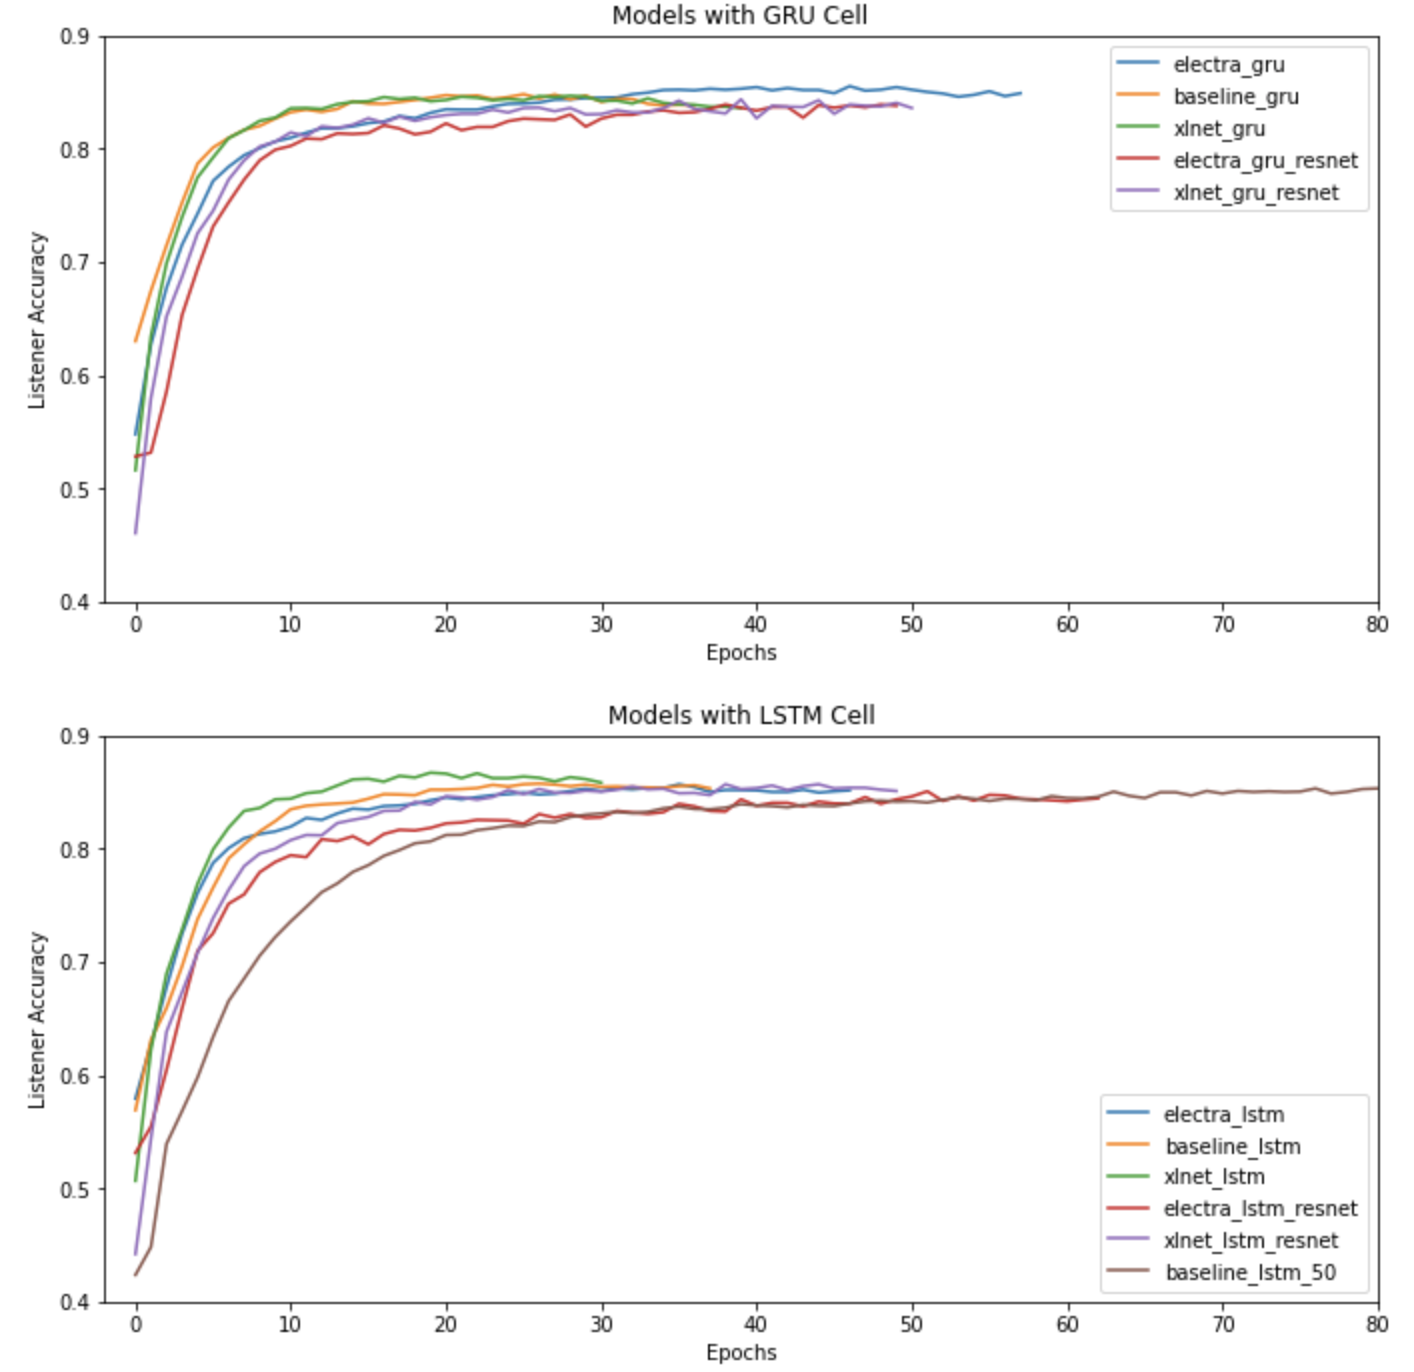
\includegraphics[width=\textwidth]{assets/learning.png}
\caption[Learning]
{Learning...}
\label{figure:learning}
\end{figure*}




% \begin{itemize}
%   \item say what experimental results mean
%   \item core conclusion
%   \item support core conclusion with error analysis, quantitative trends
%   \item describe succeedings and failings
% \end{itemize}
\section{Conclusion}

Grounded understanding presumes common world and contextual understanding of a given topic. To understand the impact of this contextual information on NLU systems we enhanced the model presented in \citep{monroe-2017-colors} with color representations encoded within convolutional neural networks such as ResNet and text descriptions represented as contextual word embeddings extracted from pretrained transformers like Electra or XLNet. We conducted a series of 80 experiments using different model setups and finetuned those models along a defined hyperparameter space.

\par
We showed that more complex color and text representations don’t necessarily perform better on the colors dataset. We find that these higher dimensional representations inject unnecessary noise to the system which leads to worse overall performance, given the low complexity of the descriptions in the color dataset.

% \begin{itemize}
%   \item briefly summarize what paper did and why
%   \item articulate broader significance of work
%   \item should be short and on point
% \end{itemize}

\section*{Acknowledgments}

We thank Prof. Christopher Potts, our course facilitator Powell Molletti and the staff of XCS224U for their guidance throughout this project.

\section*{Authorship}

All authors contributed to all project deliverables, target model development, experiment design and execution as well as final analysis and conclusive discussion.

Anton Gochev - Review of papers, transformers’ pre-trained and contextual embeddings extraction, modifications to the baseline model to support extraction of different embeddings, extension to the baseline model to support LSTM units, experiment design and execution with different hyperparameters, RNN units and embeddings, contribution to all project papers.

Jaro Habr - Baseline model implementation and finetuning, transformers embeddings research and exploration, contribution to target architecture design and end-to-end testing, experiment design and execution as well as to project coordination.

Yan Jiang - Lorem impsum

Samuel Kahn - Wrote seq2seq attention architecture, wrote convolutional color encoder for experiments, helped with high level model discussing and architectural designs, wrote analysis sections, contributed to all project papers, reviewed 4 papers.


\bibliography{references}
\bibliographystyle{acl_natbib}

\appendix
\clearpage
\section{Appendix}
\label{sec:appendix}

\begin{figure}[htb!]
  \centering
  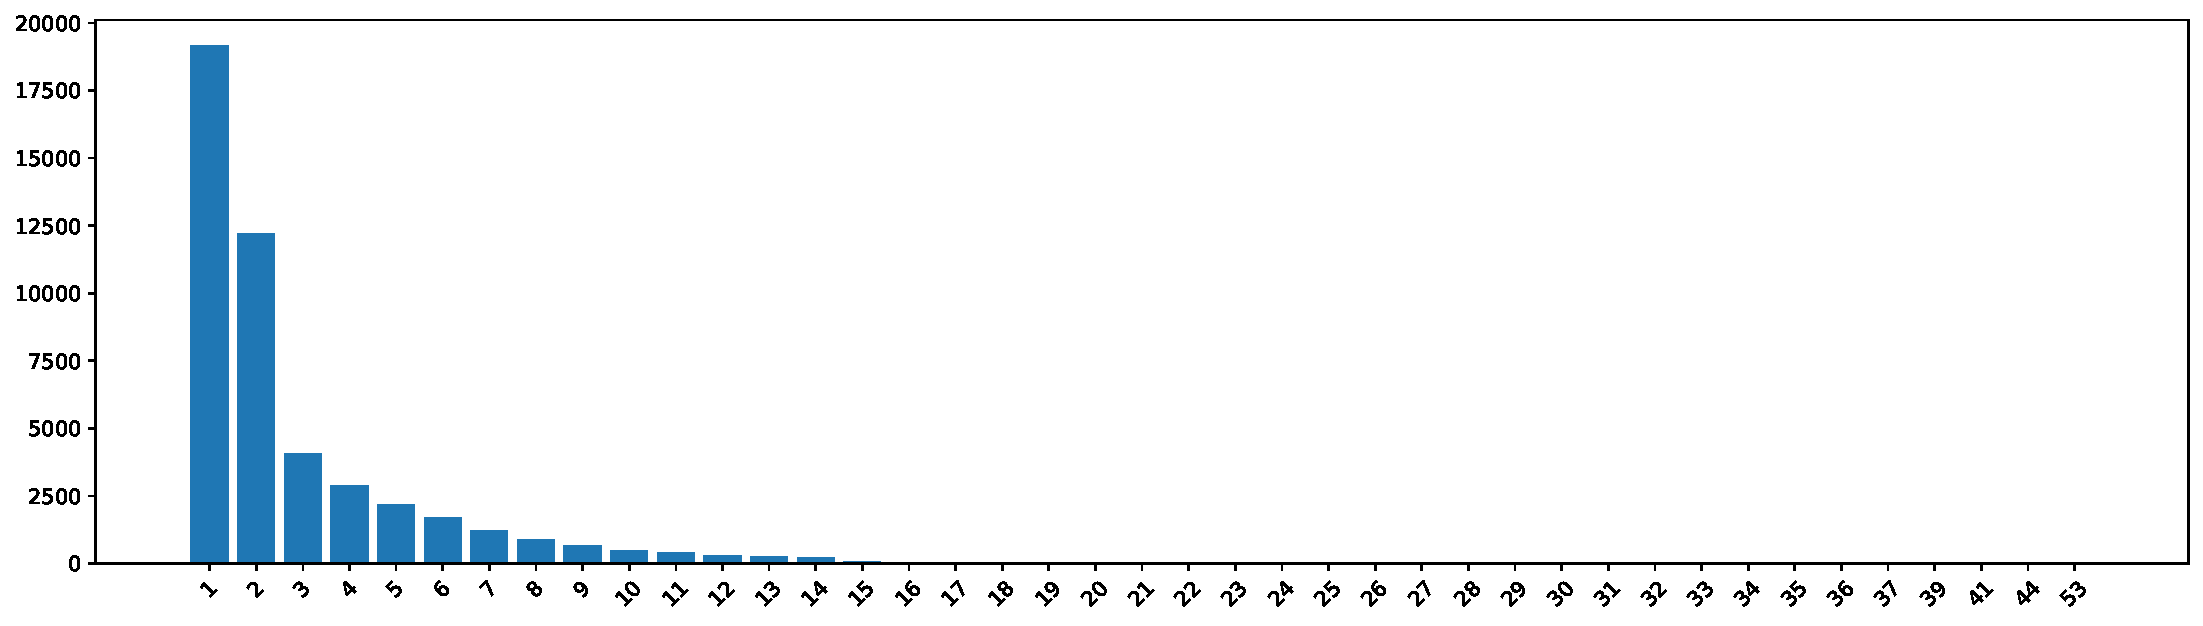
\includegraphics[width=\textwidth]{assets/trainset_words.pdf}
  \caption[Train dataset words]{Distributions of words in the train dataset.}
  \label{figure:trainset-words}
\end{figure}

\begin{figure}[htb!]
  \centering
  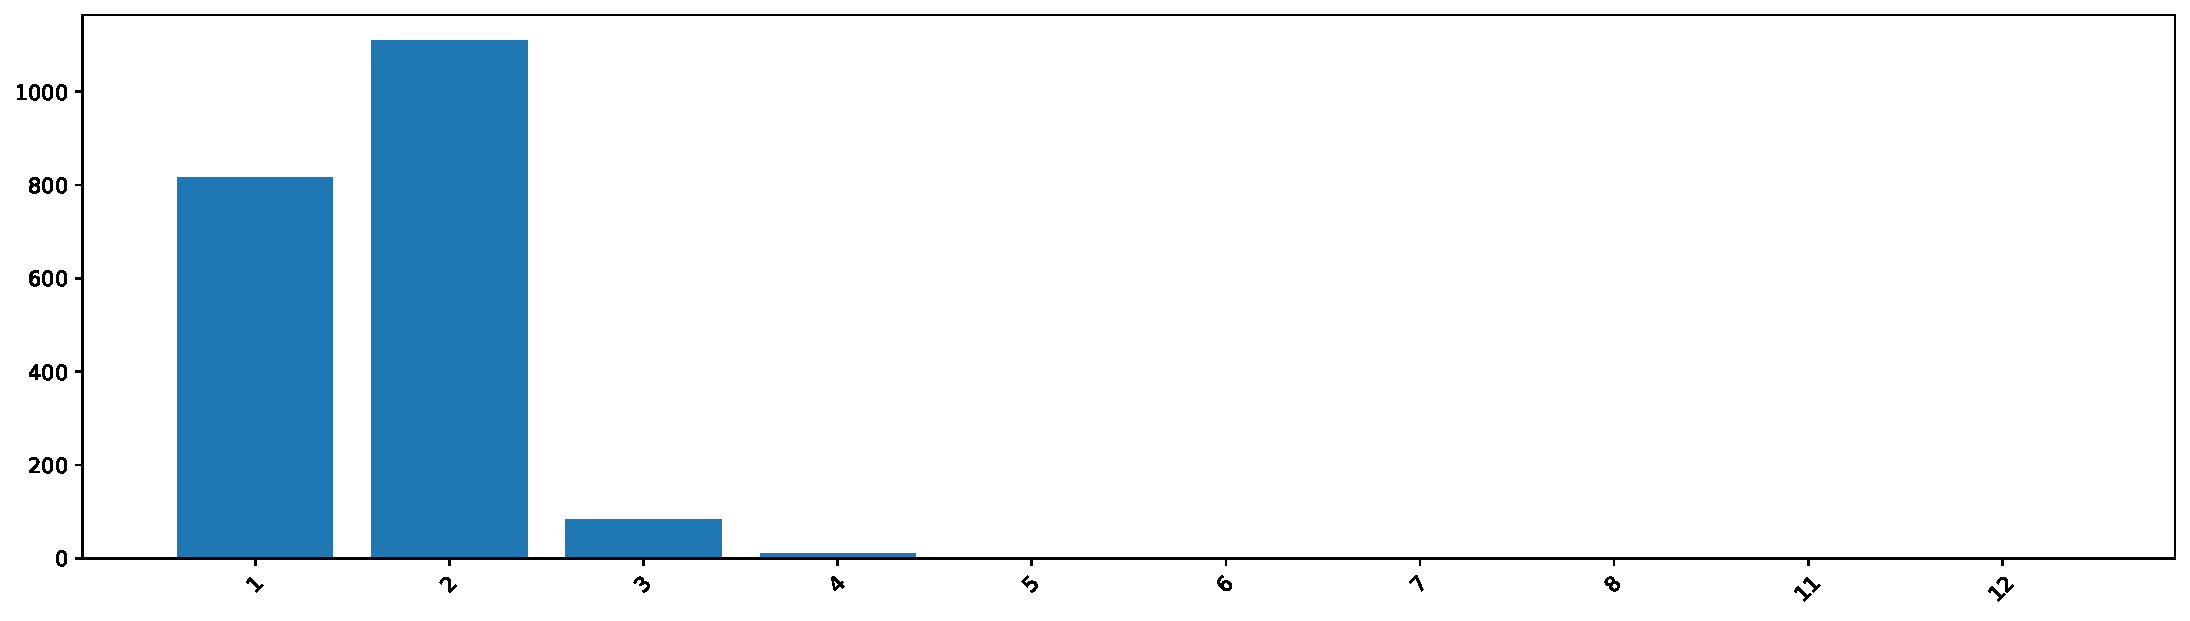
\includegraphics[width=\textwidth]{assets/testset_words.pdf}
  \caption[Test dataset words]{Distributions of words in the test dataset.}
  \label{figure:testset-words}
\end{figure}

\begin{figure}[htb!]
  \centering
  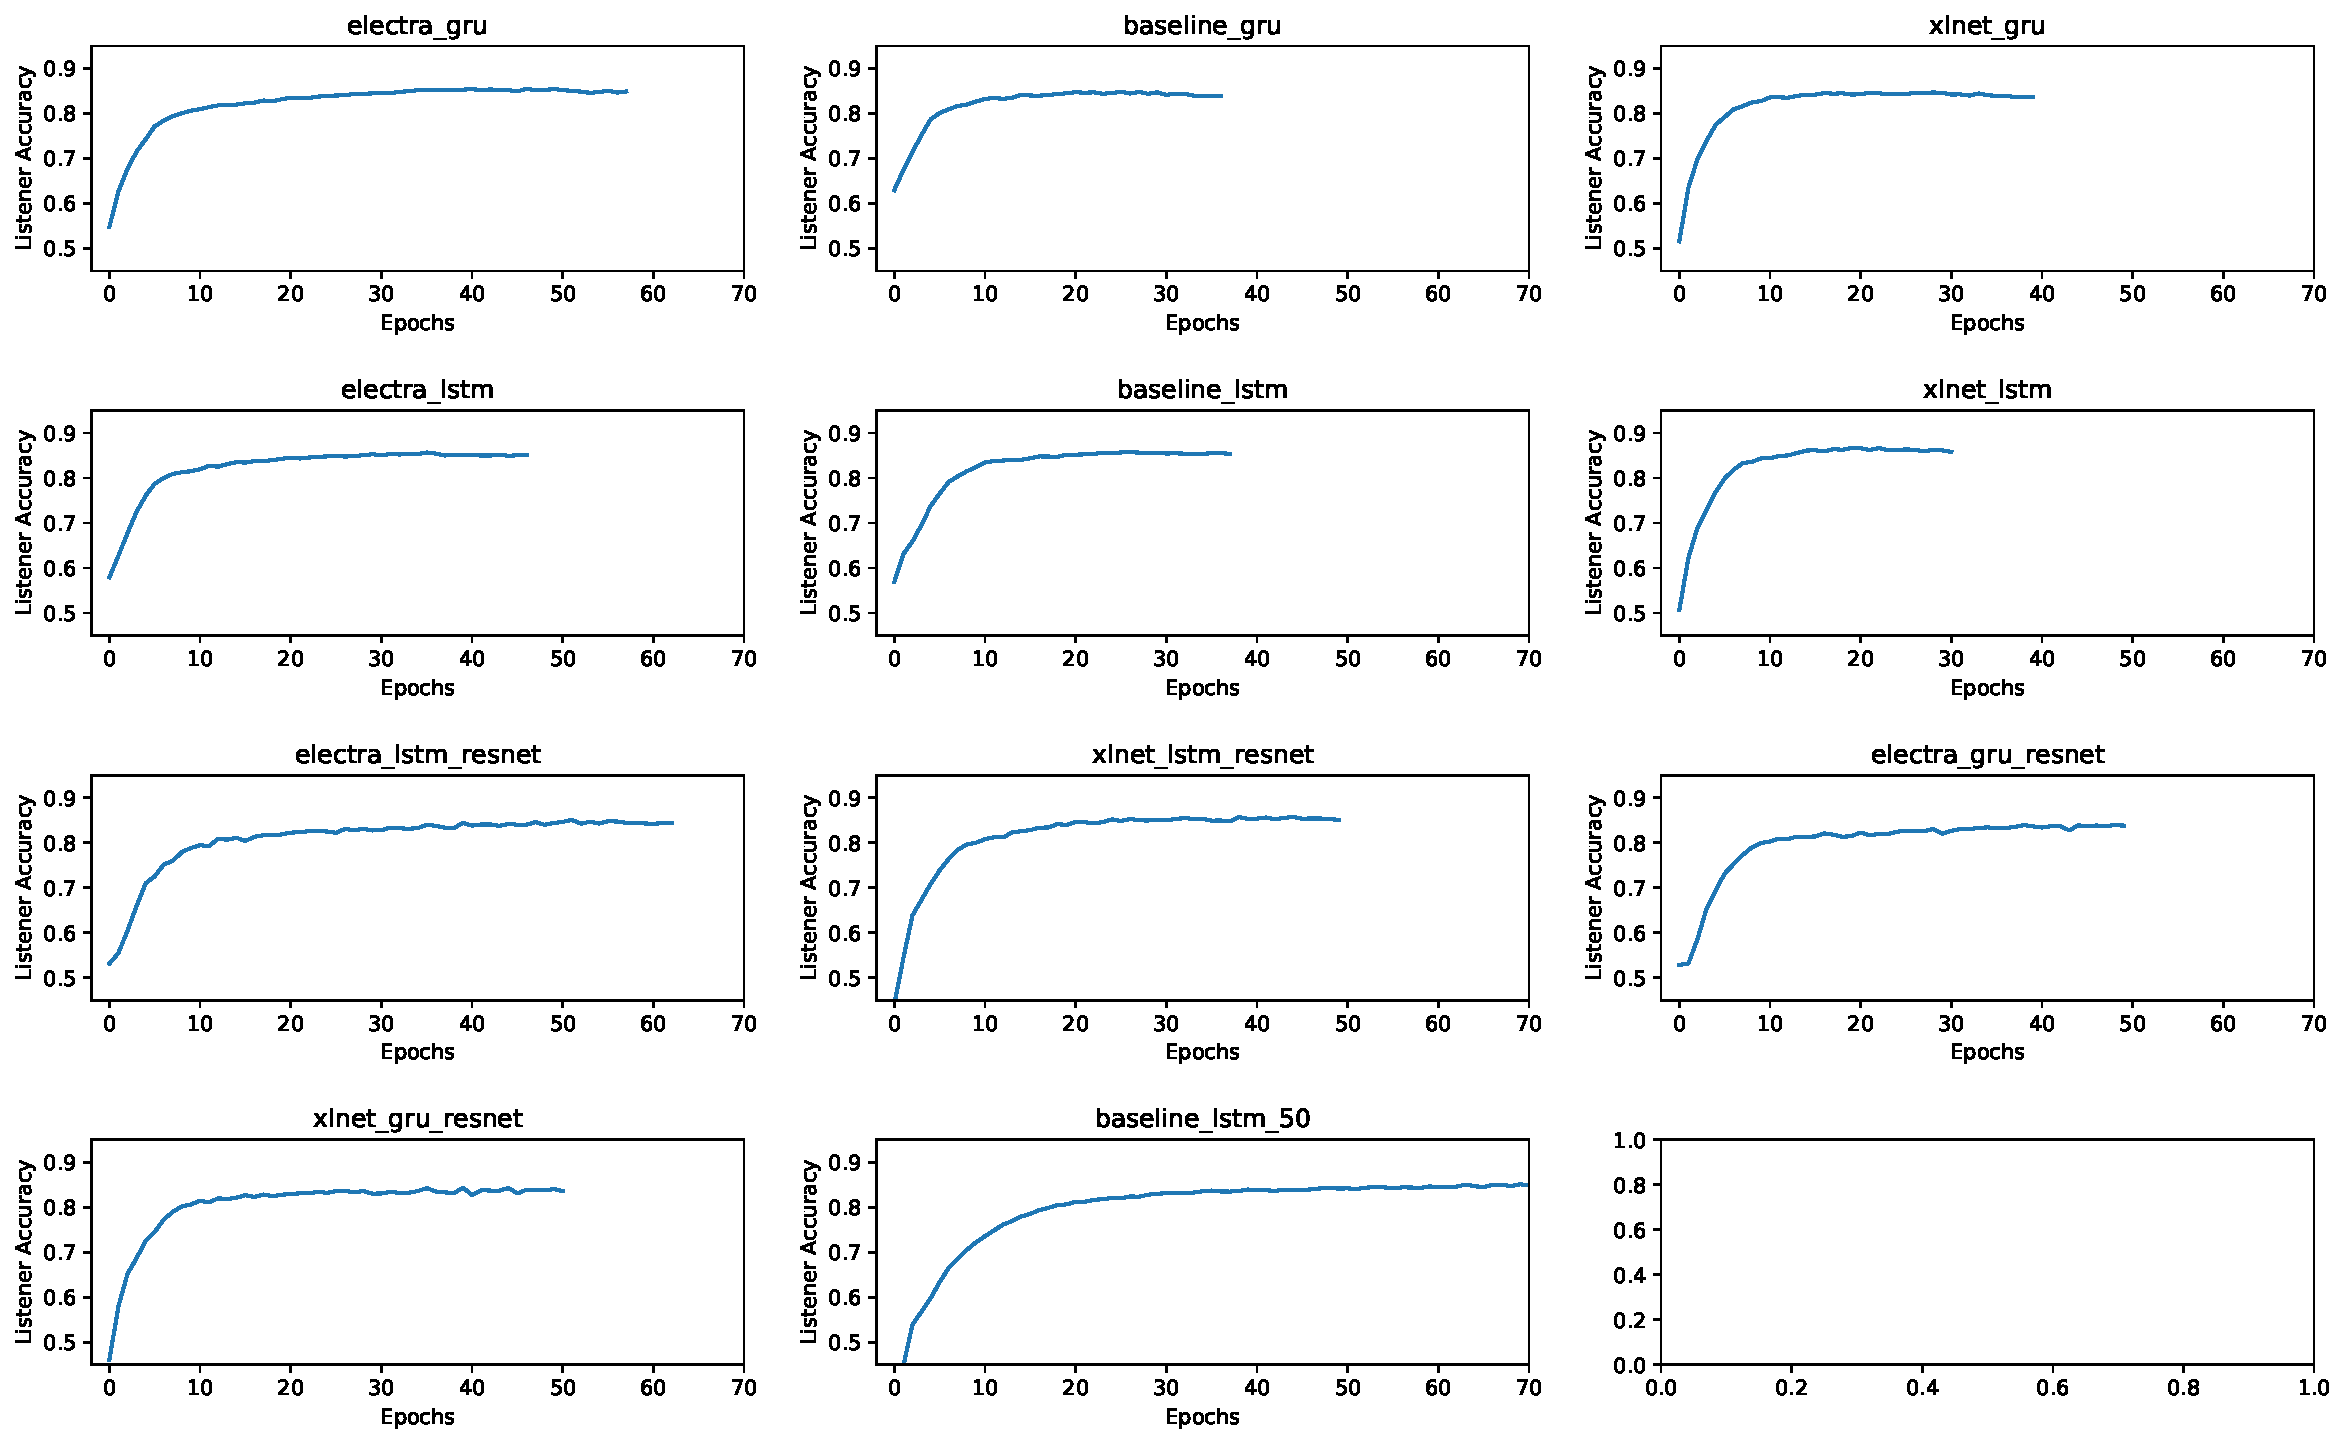
\includegraphics[width=\textwidth]{assets/training_accuracy.pdf}
  \caption[Training Accuracy]{Training accuracy.}
  \label{figure:training-accuracy}
\end{figure}

\clearpage

\begin{figure}[ht]
  \centering
  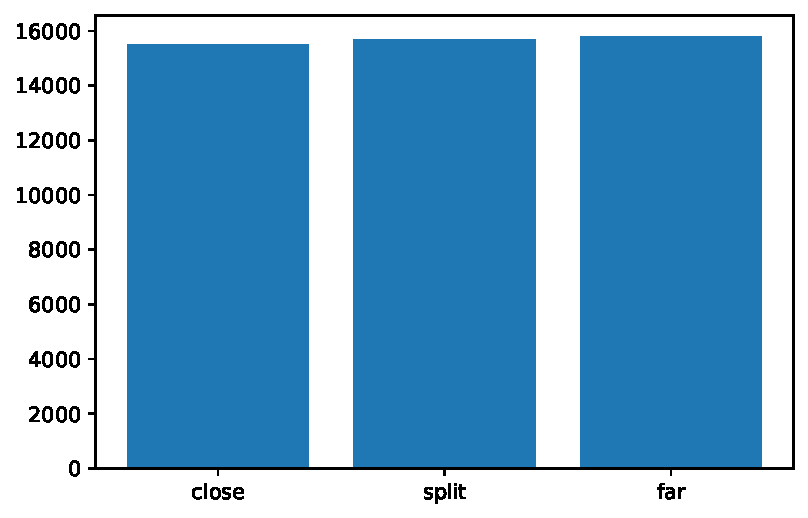
\includegraphics[width=\columnwidth]{assets/trainset_conditions.pdf}
  \caption[Train dataset words]{Distributions of conditions in the train dataset.}
  \label{figure:trainset-conditions}
\end{figure}

\begin{figure}[ht]
  \centering
  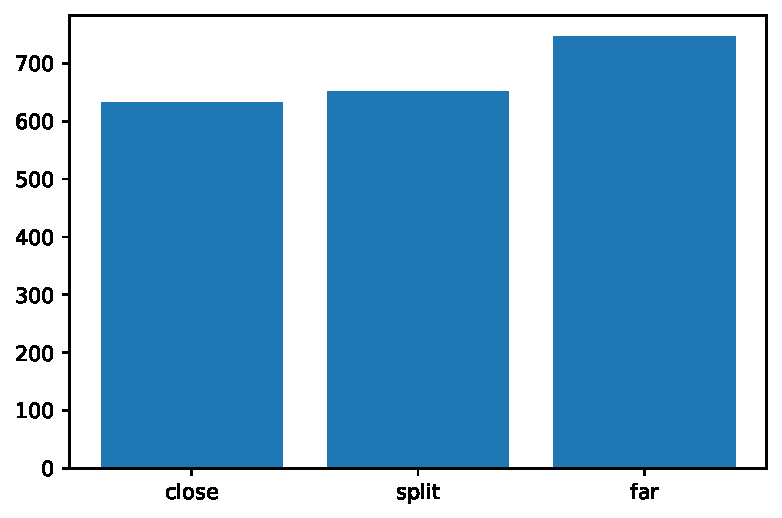
\includegraphics[width=\columnwidth]{assets/testset_conditions.pdf}
  \caption[Test dataset words]{Distributions of conditions in the test dataset.}
  \label{figure:testset-conditions}
\end{figure}


\end{document}
